\documentclass{article}
\usepackage[utf8]{inputenc}
\usepackage[spanish]{babel}
\usepackage{listings}
\usepackage{subfigure}
\usepackage{graphicx}
\usepackage{url}

\usepackage{color}


\setlength{\parindent}{0pt}
\setlength{\parskip}{1em}


\definecolor{mygreen}{rgb}{0,0.6,0}
\definecolor{mygray}{rgb}{0.5,0.5,0.5}
\definecolor{mymauve}{rgb}{0.58,0,0.82}
\lstset{ 
  backgroundcolor=\color{white},   % choose the background color; you must add \usepackage{color} or \usepackage{xcolor}; should come as last argument
  basicstyle=\footnotesize,        % the size of the fonts that are used for the code
  breakatwhitespace=false,         % sets if automatic breaks should only happen at whitespace
  breaklines=true,                 % sets automatic line breaking
  captionpos=b,                    % sets the caption-position to bottom
  commentstyle=\color{mygreen},    % comment style
  deletekeywords={...},            % if you want to delete keywords from the given language
  escapeinside={\%}{)},          % if you want to add LaTeX within your code
  extendedchars=true,              % lets you use non-ASCII characters; for 8-bits encodings only, does not work with UTF-8
  firstnumber=1,                % start line enumeration with line 1000
  frame=single,	                   % adds a frame around the code
  keepspaces=true,                 % keeps spaces in text, useful for keeping indentation of code (possibly needs columns=flexible)
  keywordstyle=\color{blue},       % keyword style
  language=Octave,                 % the language of the code
  morekeywords={*,...},            % if you want to add more keywords to the set
  numbers=left,                    % where to put the line-numbers; possible values are (none, left, right)
  numbersep=5pt,                   % how far the line-numbers are from the code
  numberstyle=\tiny\color{mygray}, % the style that is used for the line-numbers
  rulecolor=\color{black},         % if not set, the frame-color may be changed on line-breaks within not-black text (e.g. comments (green here))
  showspaces=false,                % show spaces everywhere adding particular underscores; it overrides 'showstringspaces'
  showstringspaces=false,          % underline spaces within strings only
  showtabs=false,                  % show tabs within strings adding particular underscores
  stepnumber=1,                    % the step between two line-numbers. If it's 1, each line will be numbered
  stringstyle=\color{mymauve},     % string literal style
  tabsize=2,	                   % sets default tabsize to 2 spaces
  title=\lstname                  % show the filename of files included with \lstinputlisting; also try caption instead of title
}
\title{Tarea 3}

\author{5271}
\date{\today}

\begin{document}
\maketitle

\section{Algoritimos utilizados en las mediciones}
Se seleccionaron cinco de los doce algoritmos para ejecutarlos sobre cinco de los grafos de tareas anteriores, midiendo los tiempos de ejecución de cada algoritmo y realizando un análisis de los datos obtenidos. Dado los requerimientos de los algoritmos escogidos para la realización de esta tarea, se tuvo modificar los dichos grafos agregándoles más nodos y se convirtiéndolos a grafos no dirigidos, como se muestra en la figura 1.
 
Los algoritmos escogidos fueron los siguientes:

\begin{itemize}
 \item\textit{Make max clique graph} (encuentra las camarillas máximas y las trata como vértices . Los vértices  están conectados si tienen miembros comunes en el grafo original)  \cite{mc}.  
 \item\textit{Betweenness centrality} (calcula la centralidad de intermediación de ruta más corta para los vértices . La centralidad de la intermediación es una forma de detectar la cantidad de influencia que un vértice tiene sobre el flujo de información en un grafo) \cite{bct}.
	\item\textit{Greedy color} (colorea un grafo usando varias estrategias de coloración codiciosa. Las estrategias se pueden describir como el intento de colorear un grafo con la menor cantidad de colores posibles, donde ningún vecino puede tener el mismo color) \cite{gc}.
	\item\textit{Maximal matching} (encuentra una cardinalidad máxima de coincidencia en el grafo. Una coincidencia es un subconjunto de aristas en las que no se produce ningún vértice más de una vez. La cardinalidad de una coincidencia es el número de arcos coincidentes. Se uso este algoritmo en lugar del\textit{min maximal matching} ya que este daba un error en networkx)\cite{mm}.
	\item\textit{Dfs tree} (crea un árbol orientado hacia el retorno construido a partir de una fuente en una búsqueda en profundidad) \cite{dt}.
\end{itemize}
\begin{center}
\lstinputlisting[language=Python, firstline=1, lastline=36]{Genera_grafos.py}
\end{center}
\begin{figure}[h]

\subfigure[grafo1, 520 vértices, 2237 aristas]{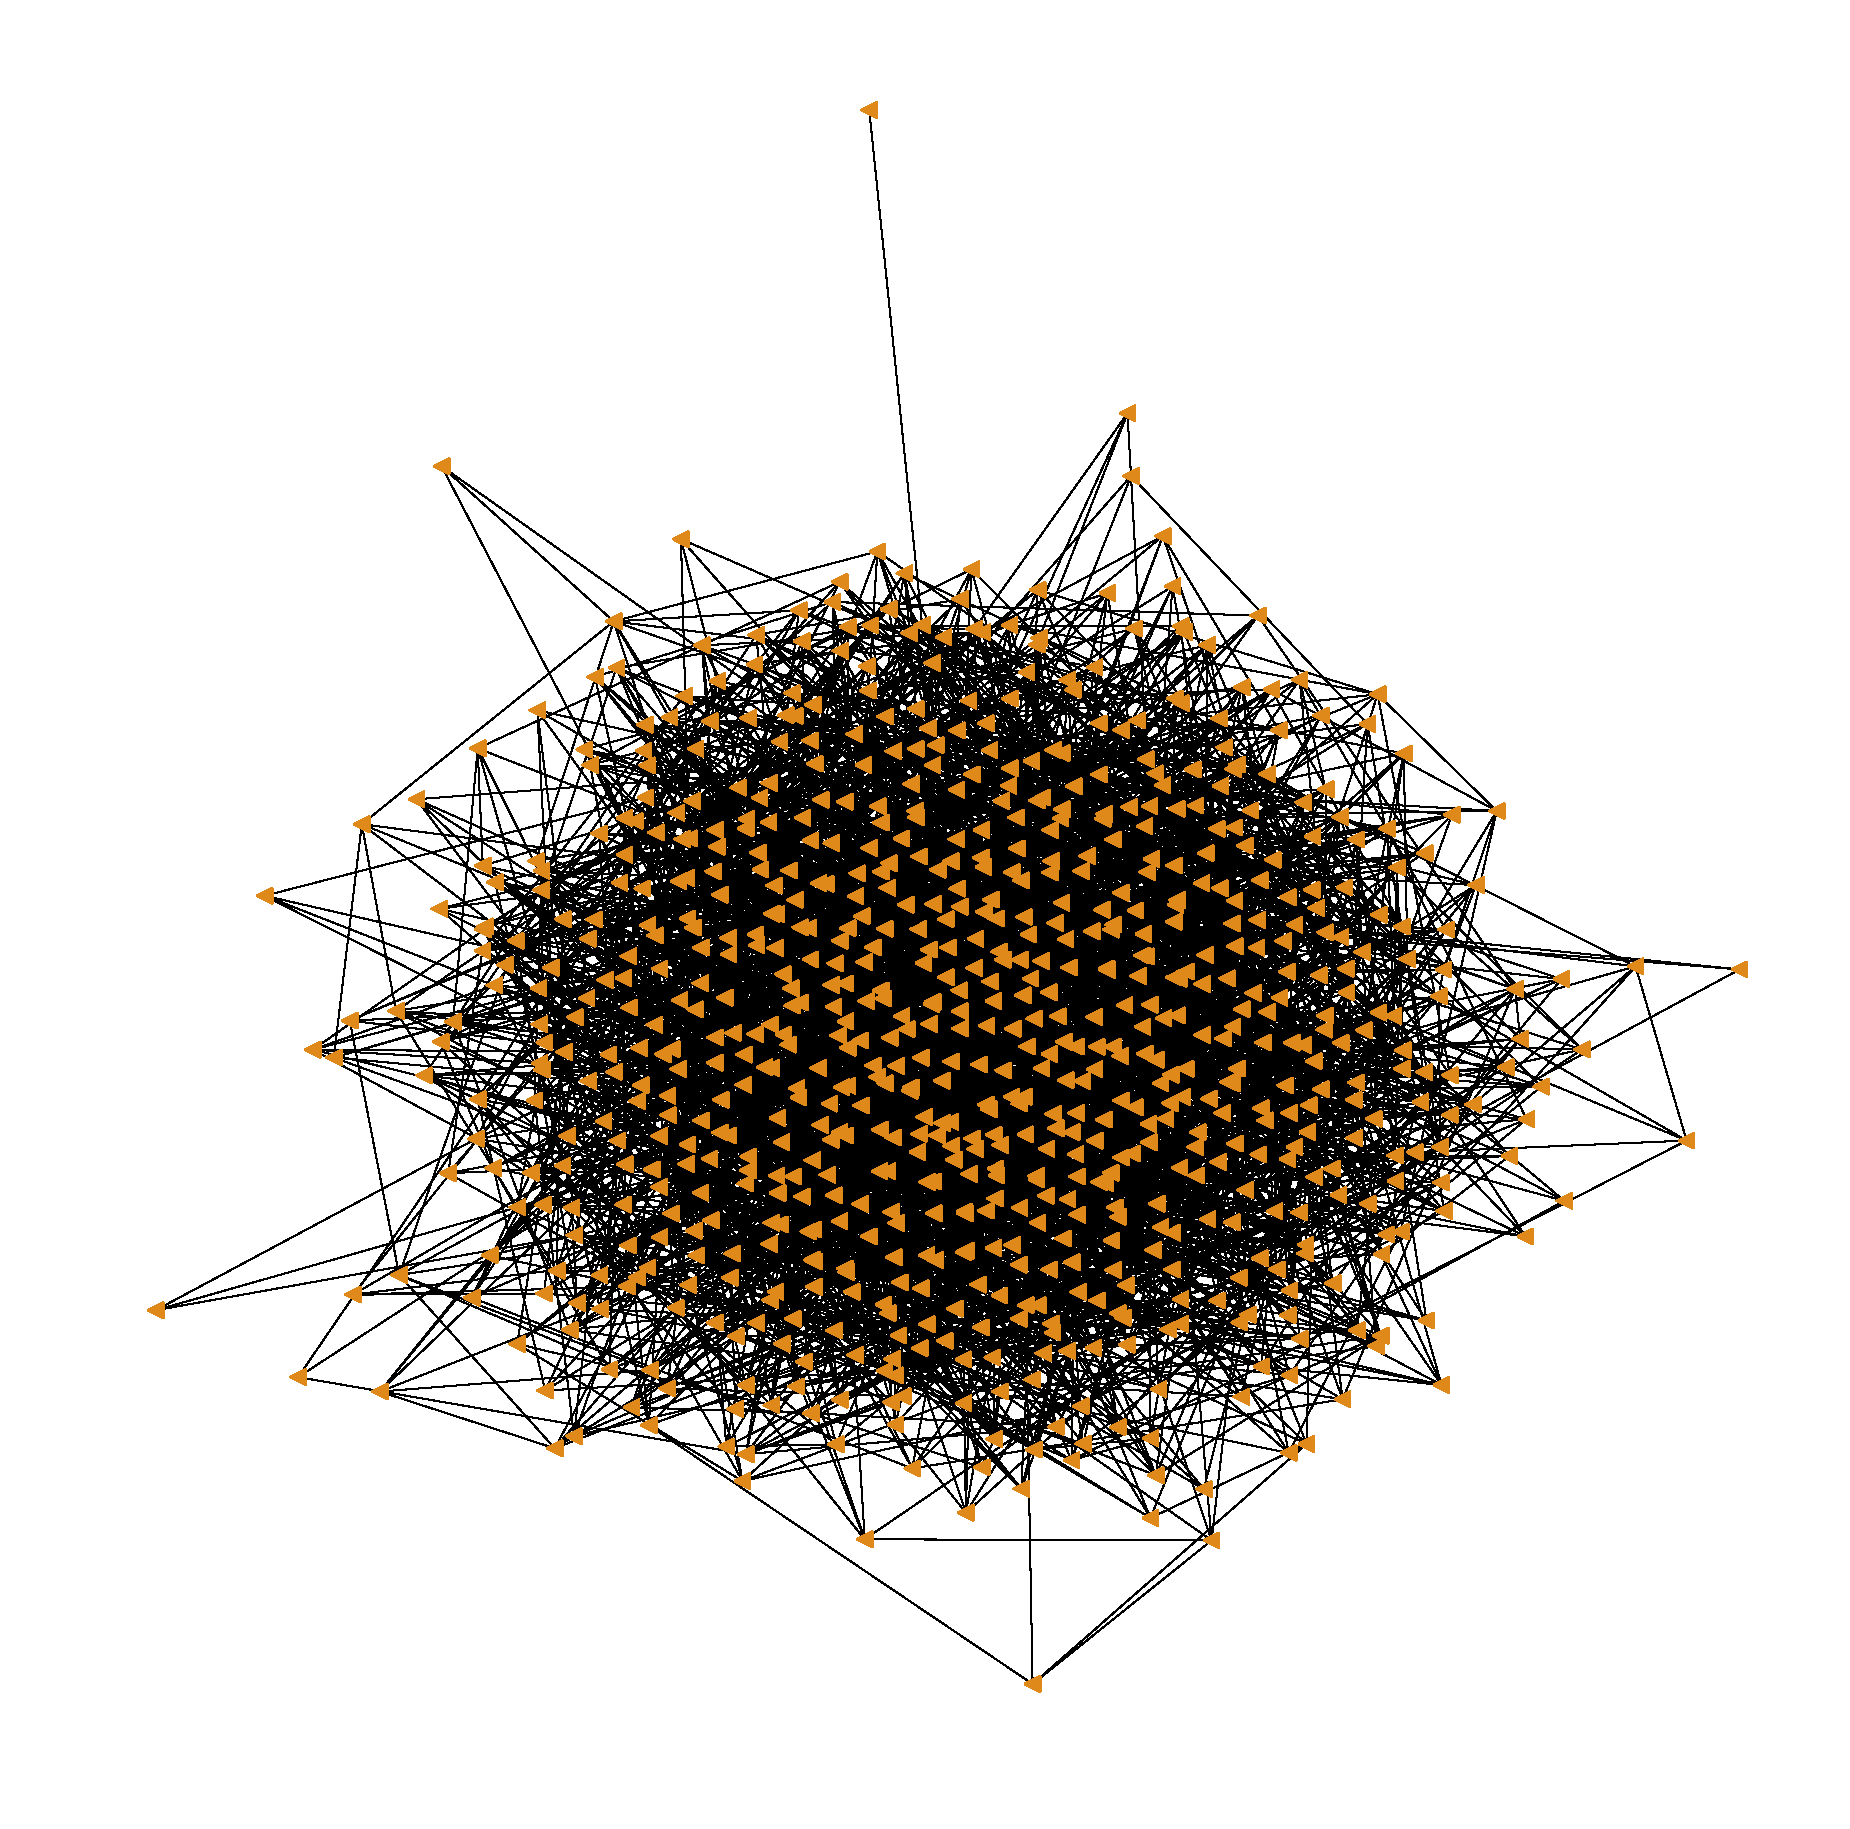
\includegraphics[scale=0.2]{1NoDirigido.eps}}
\subfigure[grafo2, 400 vértices, 1241 aristas]{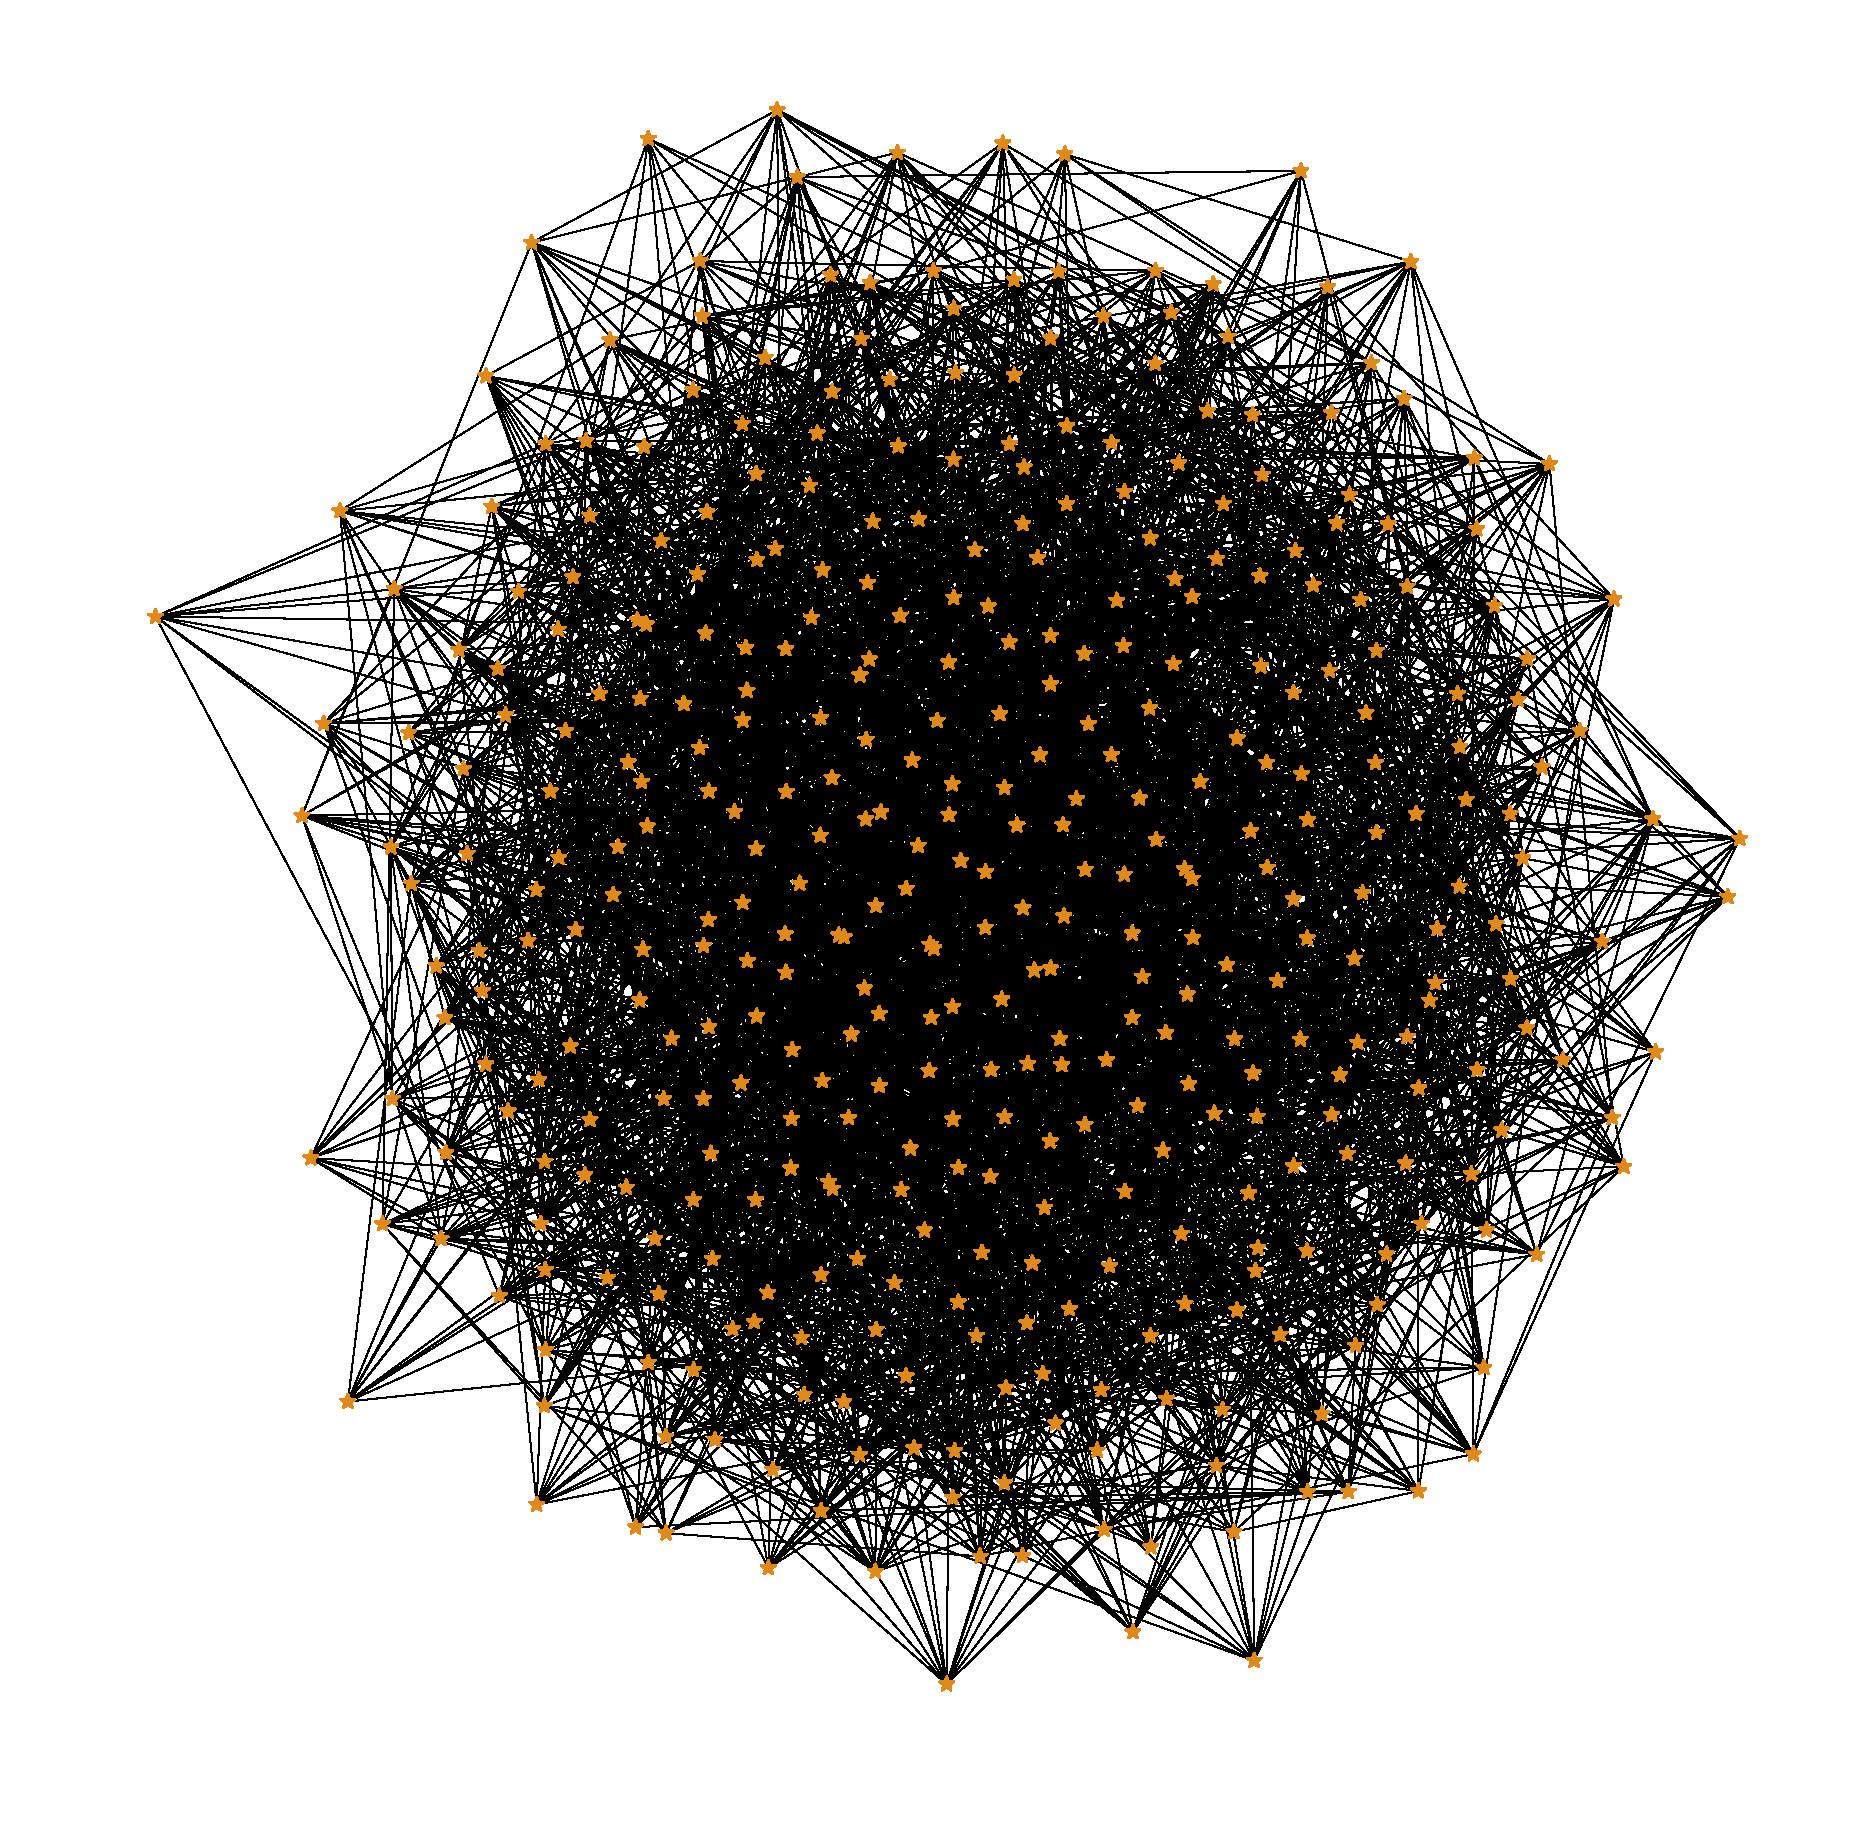
\includegraphics[scale=0.2]{2NoDirigido.eps}}
\subfigure[grafo3, 350 vértices, 1963 aristas]{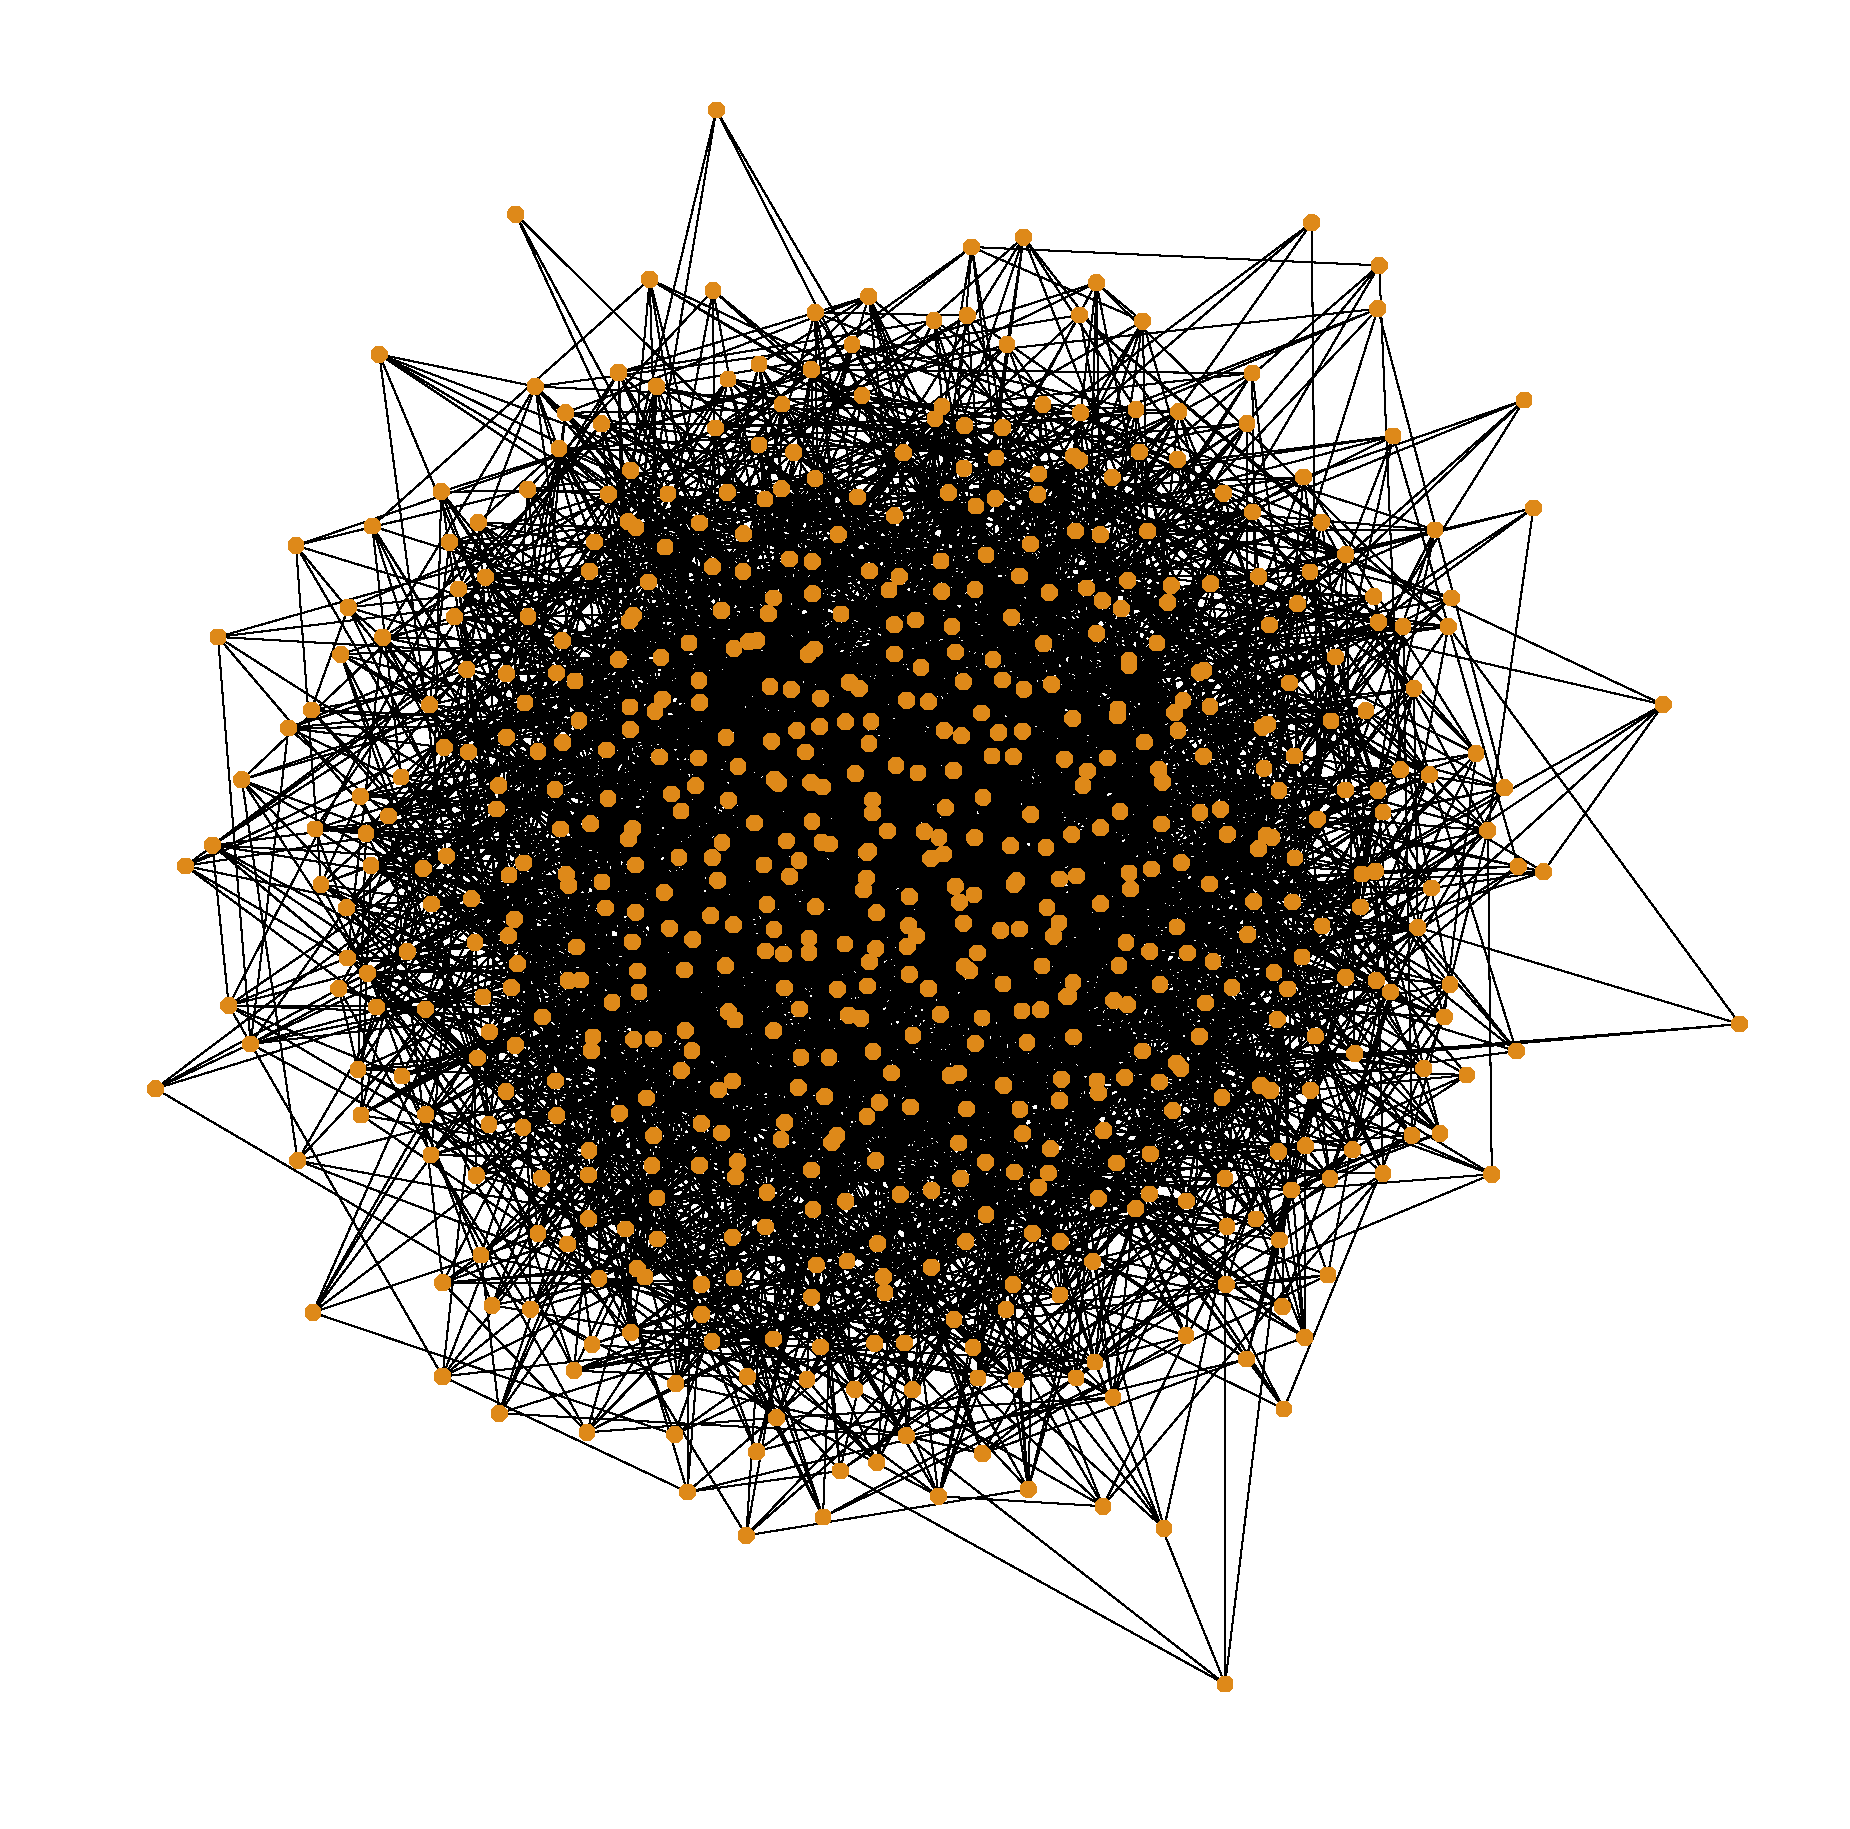
\includegraphics[scale=0.2]{3NoDirigido.eps}}
\subfigure[grafo4, 749 vértices, 2767 aristas]{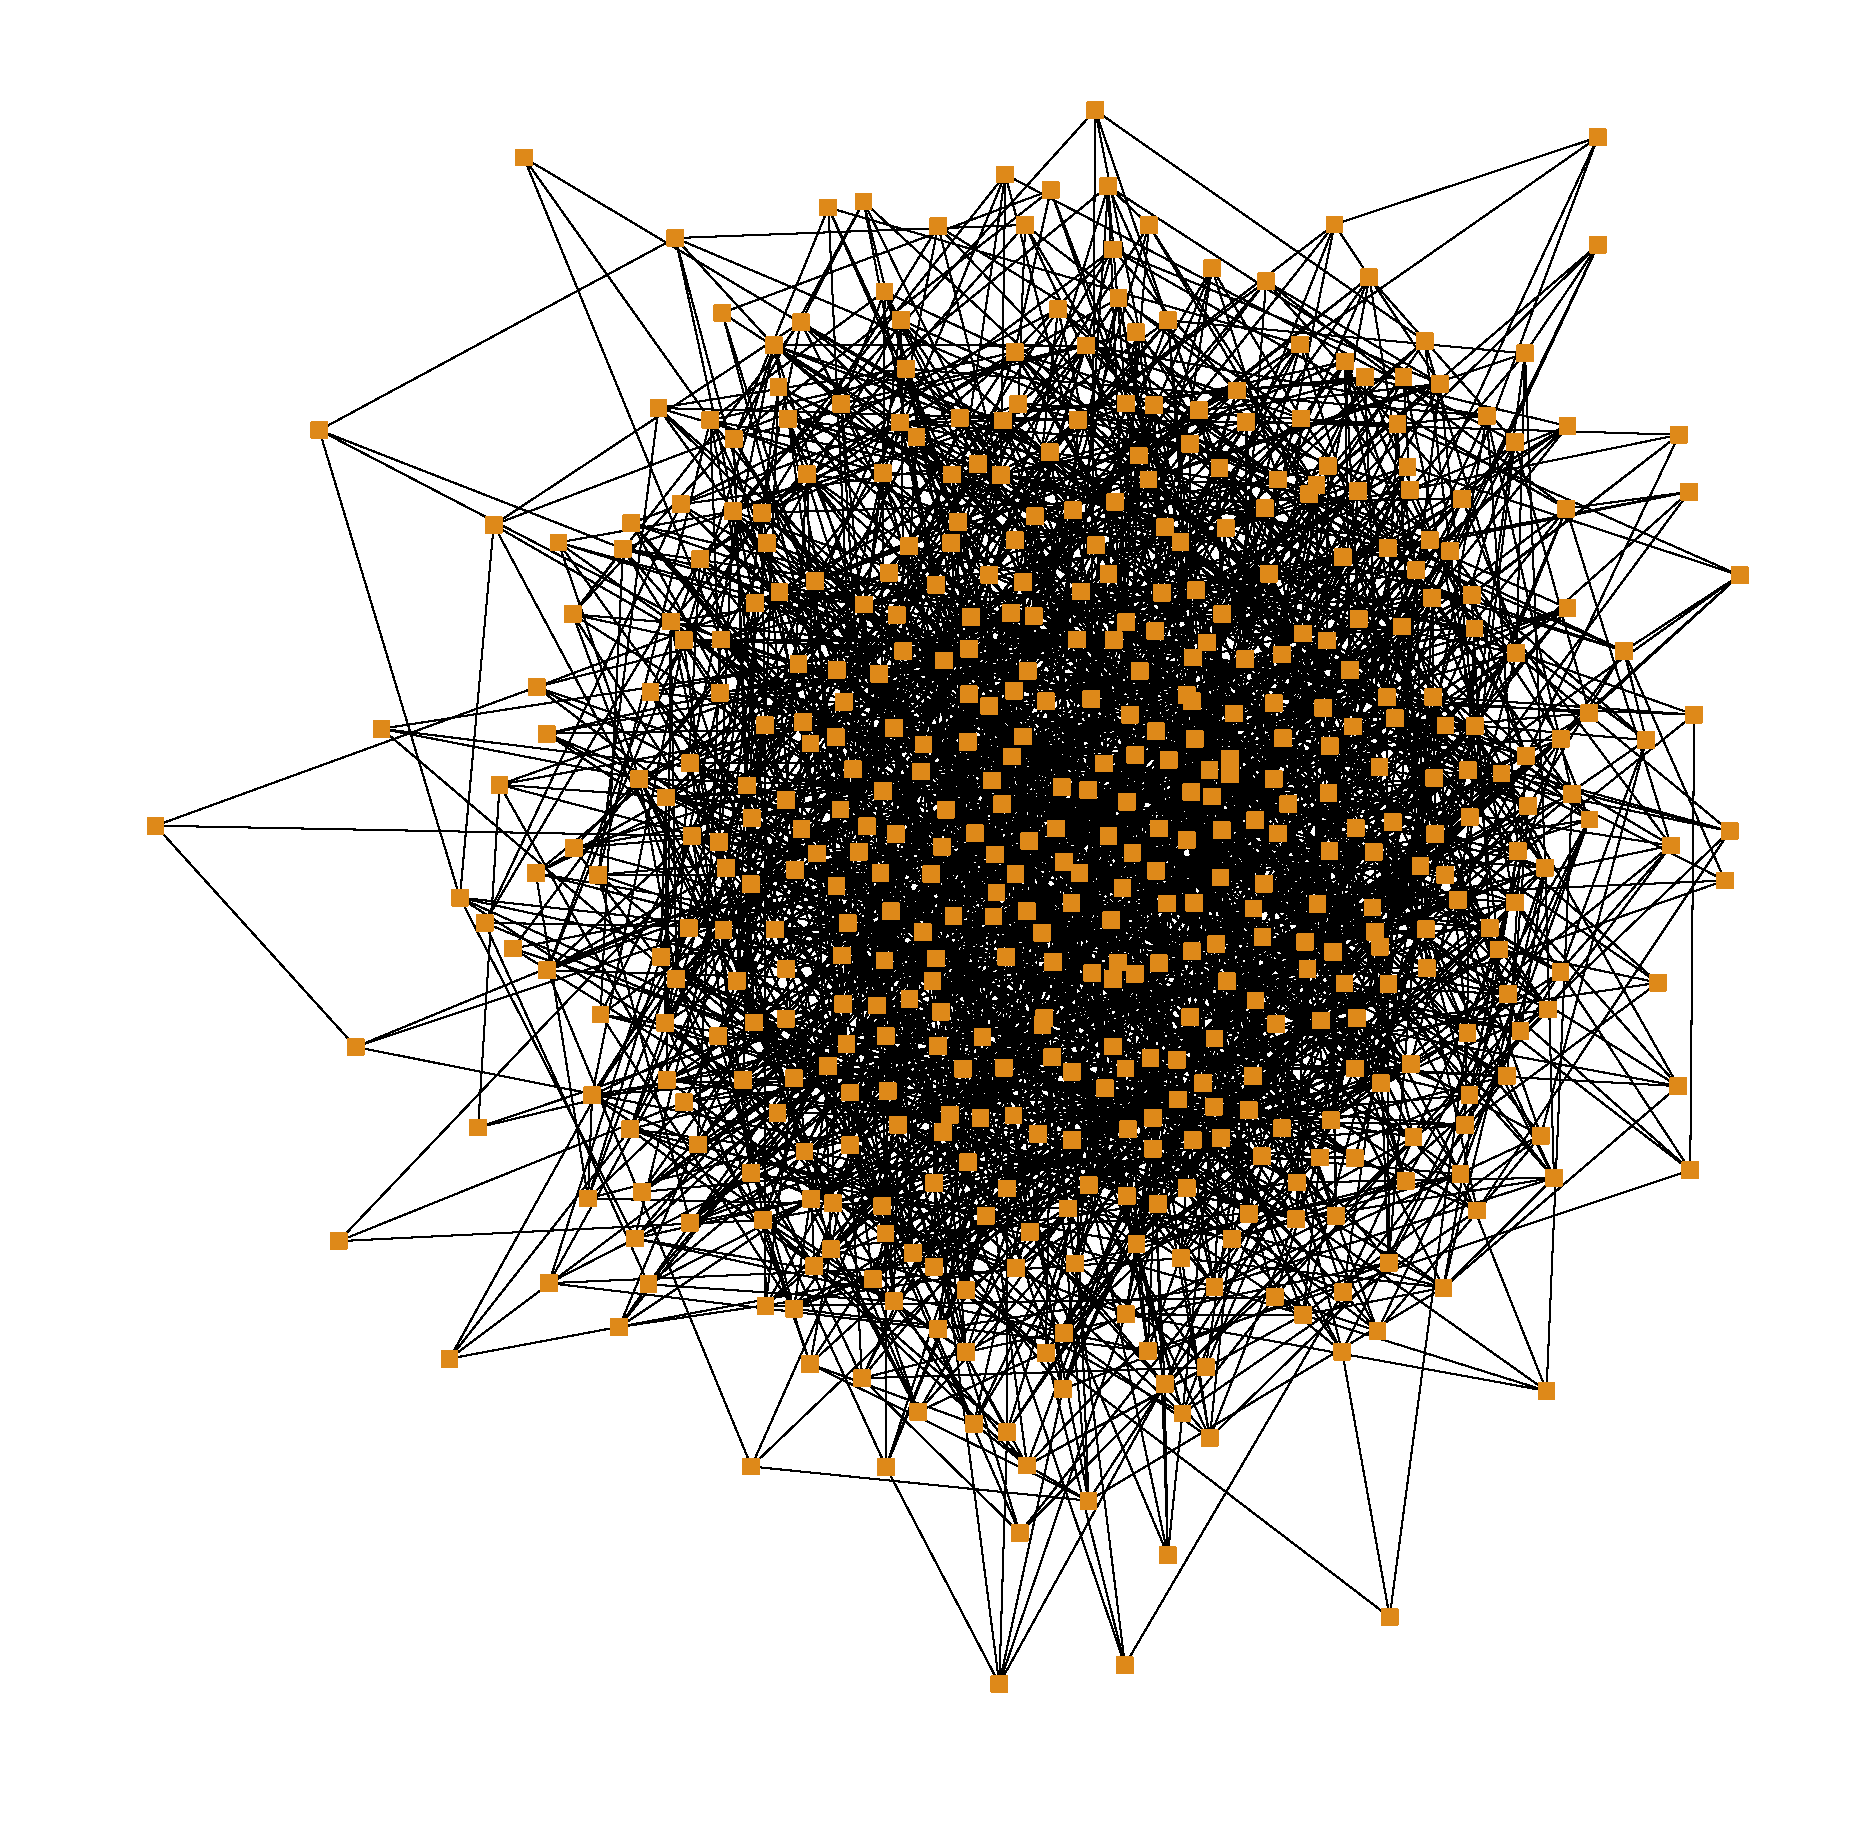
\includegraphics[scale=0.2]{4NoDirigido.eps}}
\subfigure[grafo5, 709 vértices, 2567 aristas]{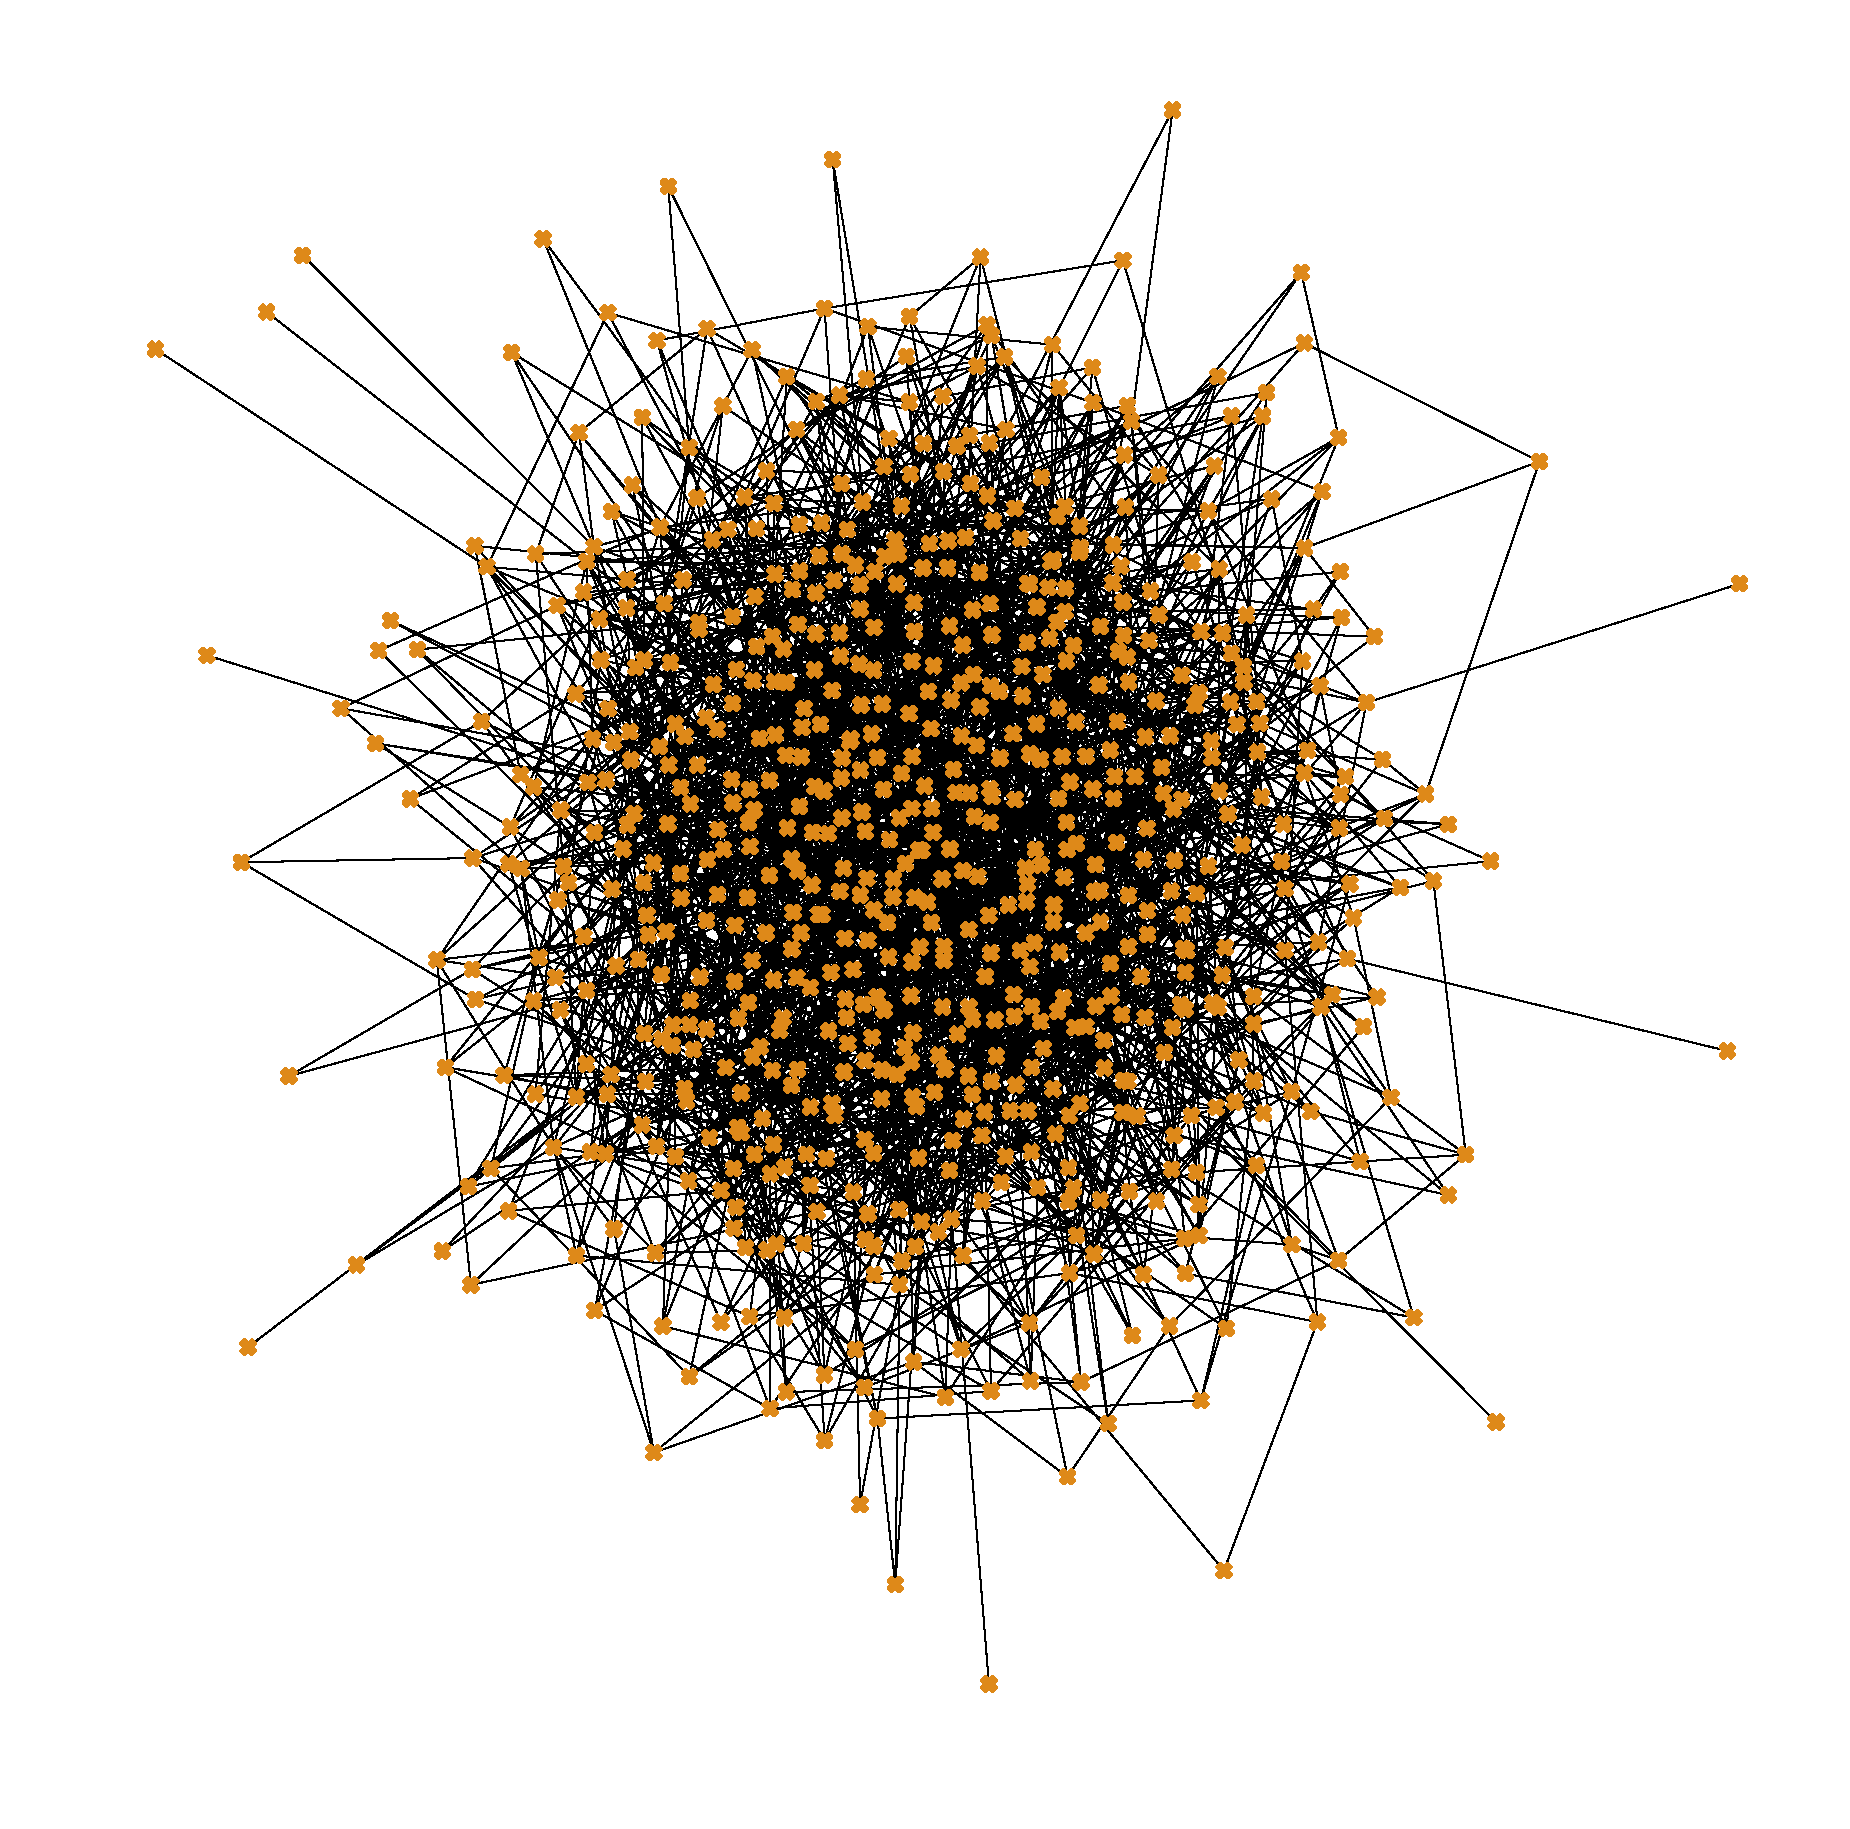
\includegraphics[scale=0.2]{5NoDirigido.eps}}

\caption{Grafos generados para la tarea 3.} 
\end{figure}
\newpage
\section{Medición de los tiempos de ejecución}
Con el objetivo de realizar las mediciones de los tiempos de ejecución de los algoritmos seleccionados se desarrolló el siguiente código.

En primer lugar, se crea una función que lee de un archivo la matriz de adyacencia de un grafo y convierte dicha matriz en un grafo.
\begin{center}
\lstinputlisting[language=Python, firstline=20, lastline=25]{Corer_Algoritmos.py}
\end{center}
Se crea una función para cada algoritmo. En esta se le pasa el grafo leído por parámetros al algoritmo en cuestión, en este proceso se mide el tiempo de ejecución del algoritmo y se repite treinta veces la ejecución, los tiempos son almacenados en una lista. Con las mediciones acumuladas se calcula la media, la mediana y la desviación estándar.
 \begin{center}
\lstinputlisting[language=Python, firstline=57, lastline=100]{Corer_Algoritmos.py}
\end{center}
En este otro fragmento se muestra donde se ejecutan las funciones y se guarda el archivo con los datos recopilados.
 \begin{center}
\lstinputlisting[language=Python, firstline=146, lastline=165]{Corer_Algoritmos.py}
\end{center}


\newpage
\section{Resultados del Análisis de los datos}

Con los datos recopilado de las ejecuciones de los Algoritmos par los cinco grafos se realizó un histograma, como se muestra en la figura 2 y dos diagramas de dispersión, uno que muestra la relación de la media de los tiempos de ejecución de cada algoritmo con la cantidad de vértices y el otro con la cantidad de aristas, como se muestra en la figura 3 y 4 respectivamente. En estas figuras se puede observar que el algoritmo con los tiempos de ejecución más pequeños es el \textit{Maximal matching}, así como que el de mayores tiempos es el \textit{Betweenness centrality}. 



  
\begin{center}
\lstinputlisting[language=Python, firstline=6, lastline=34]{Histograma.py}
\end{center}

\newpage
\begin{center}
\lstinputlisting[language=Python, firstline=37, lastline=61]{Histograma.py}
\end{center}

\begin{figure}[h]

\includegraphics[scale=0.6]{Histograma.eps}
\caption{Histograma que de los cinco algoritmos con cinco grafos.}
\end{figure}
\begin{figure}[h]
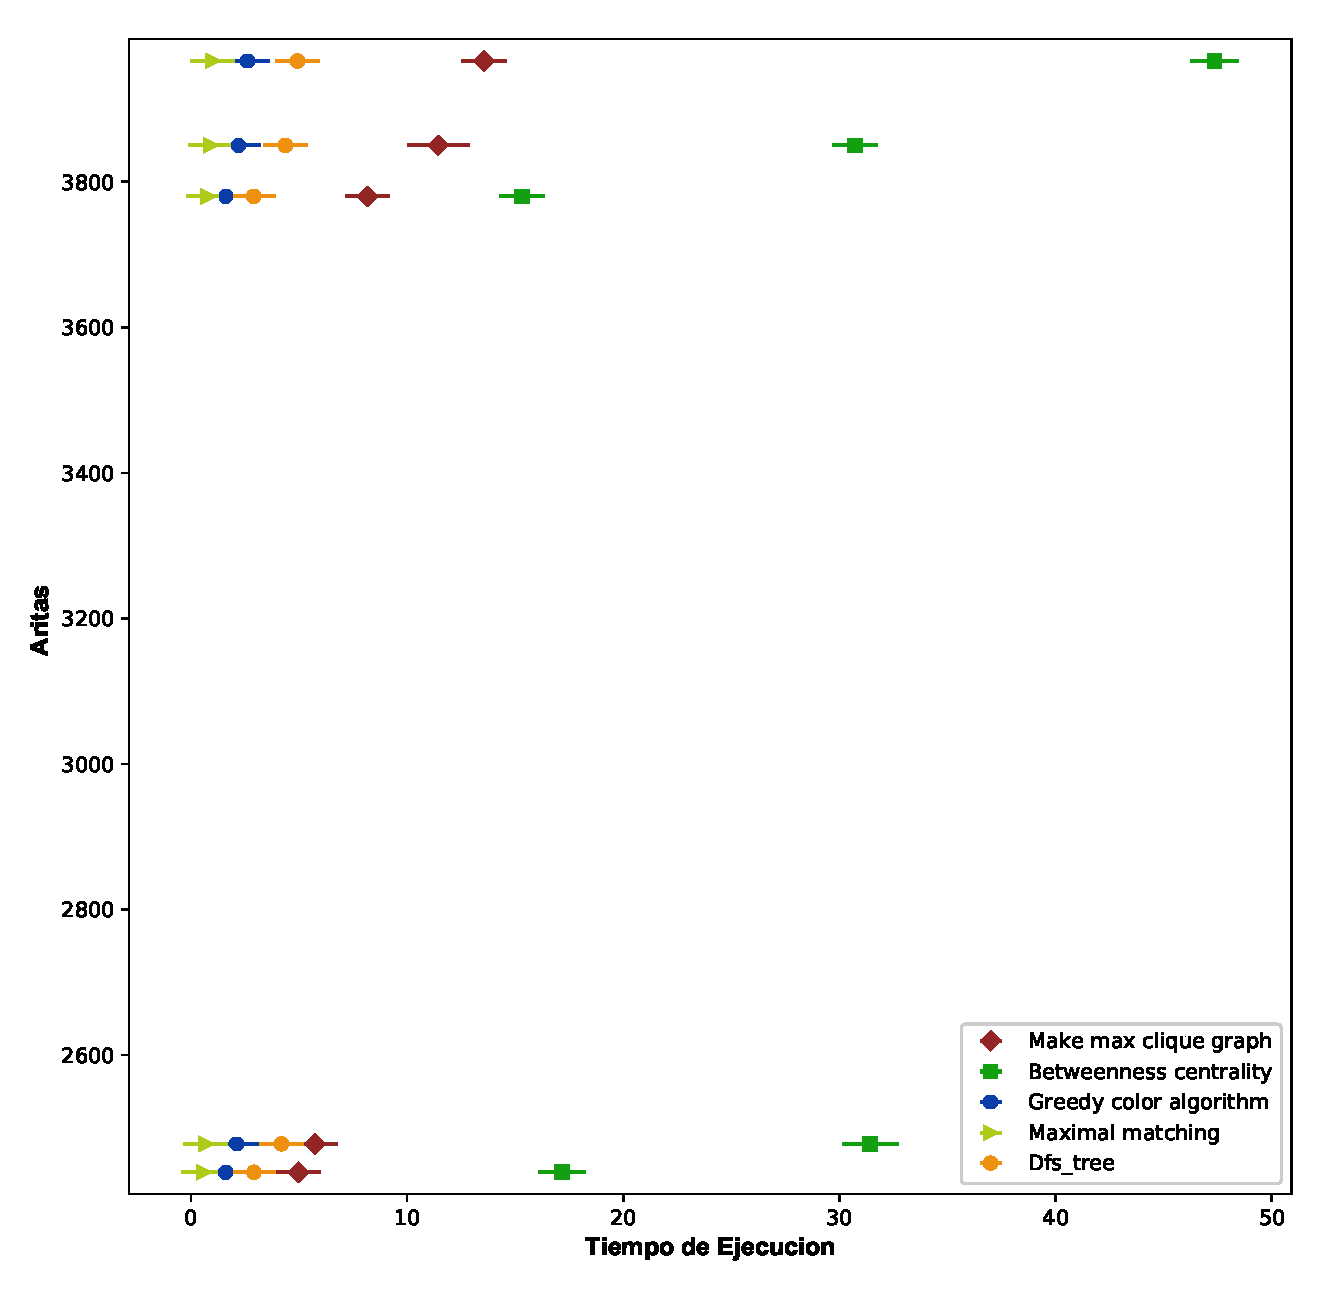
\includegraphics[scale=0.6]{DiagramAristas.eps}
\caption{Diagrama de dispersión que muestra la relación entre los tiempos de ejecución y la cantidad de vértices.}
\end{figure}
\begin{figure}[h]
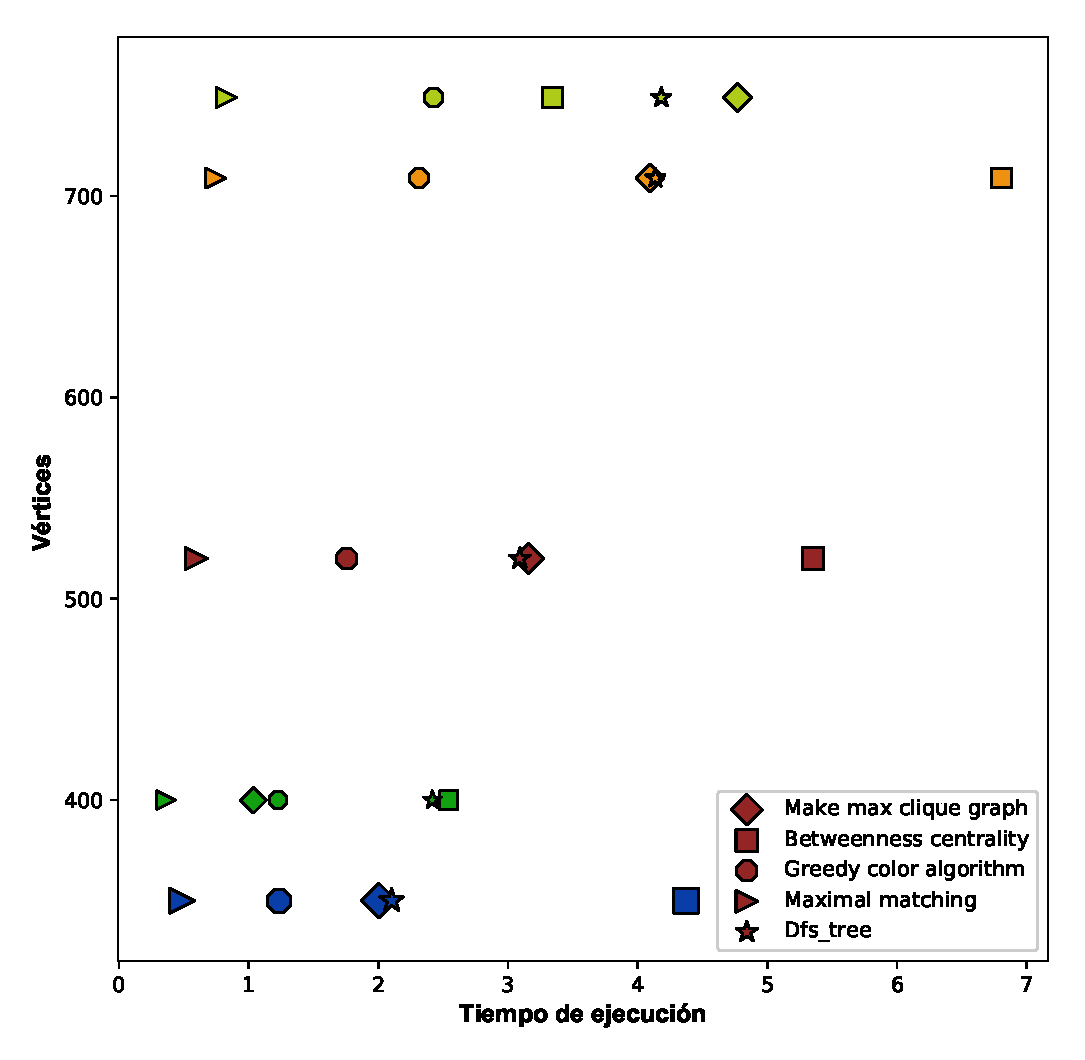
\includegraphics[scale=0.6]{DiagramVertices.eps}
\caption{Diagrama de dispersión que muestra la relación entre los tiempos de ejecución y la cantidad de aristas.}
\end{figure}
 
\newpage

\newpage
\bibliography{tarea3}
\bibliographystyle{plain}
\end{document}
